\section{Hardware Setup/implementation}
\subsection{System Architecture}

\begin{figure}[h]
  \centering
  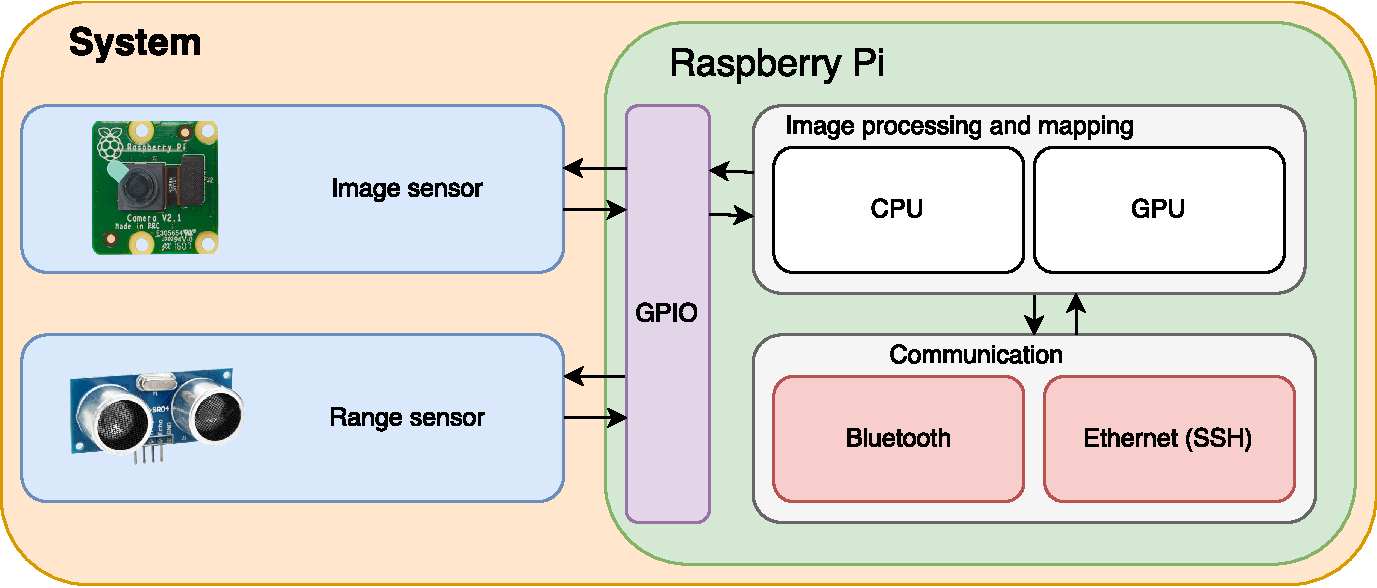
\includegraphics[width=1\textwidth]{fig/system}
  \caption{System architecture}
  \label{fig:system}
\end{figure}

The overall system architecture is illustrated in Figure \ref{fig:system}. With the exception of a power source and memory, this is a view simplification of the system interconnections. The sensors are connected through the GPIO interface on the Raspberry Pi, and all the image processing is done internally in the CPU/GPU.

\subsection{System Setup}
Figure \ref{fig:setup_n} and \ref{fig:setup_d} shows the complete system in a picture of how the all the hardware is connected for normal operation and for debugging. Since the Raspberry Pi is running Raspbian OS which features a GUI, debugging can be done on a monitor with USB peripherals connected such as a keyboard and mouse. During normal operation however, the system should not be connected to anything else than power and a communication protocol. \\

I will describe each component of this system closer in this section.

\begin{figure}[H]
  \centering
  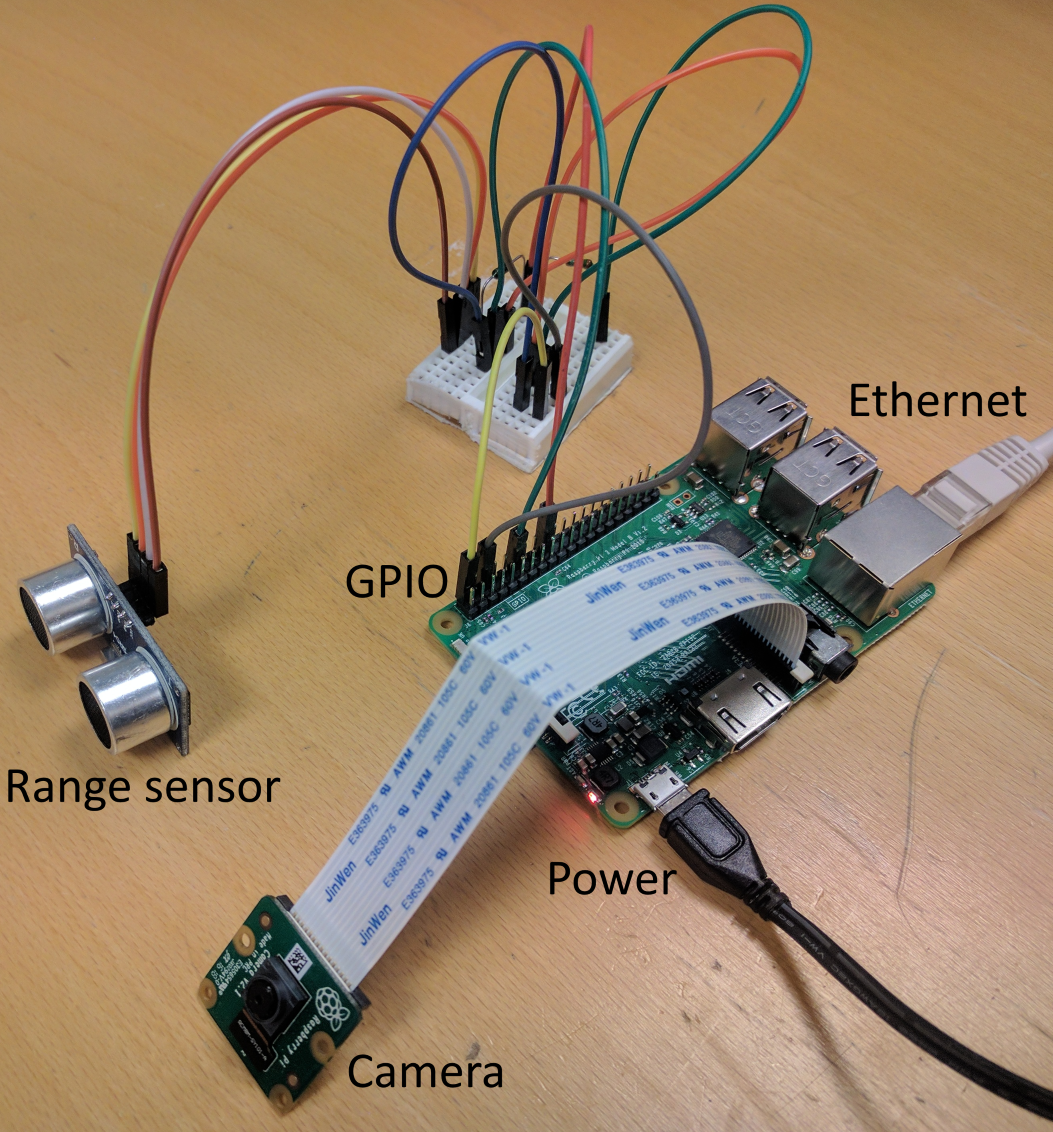
\includegraphics[width=0.85\textwidth]{fig/setup_normal}
  \caption{Normal hardware setup}
  \label{fig:setup_n}
\end{figure}
\begin{figure}[H]
  \centering
  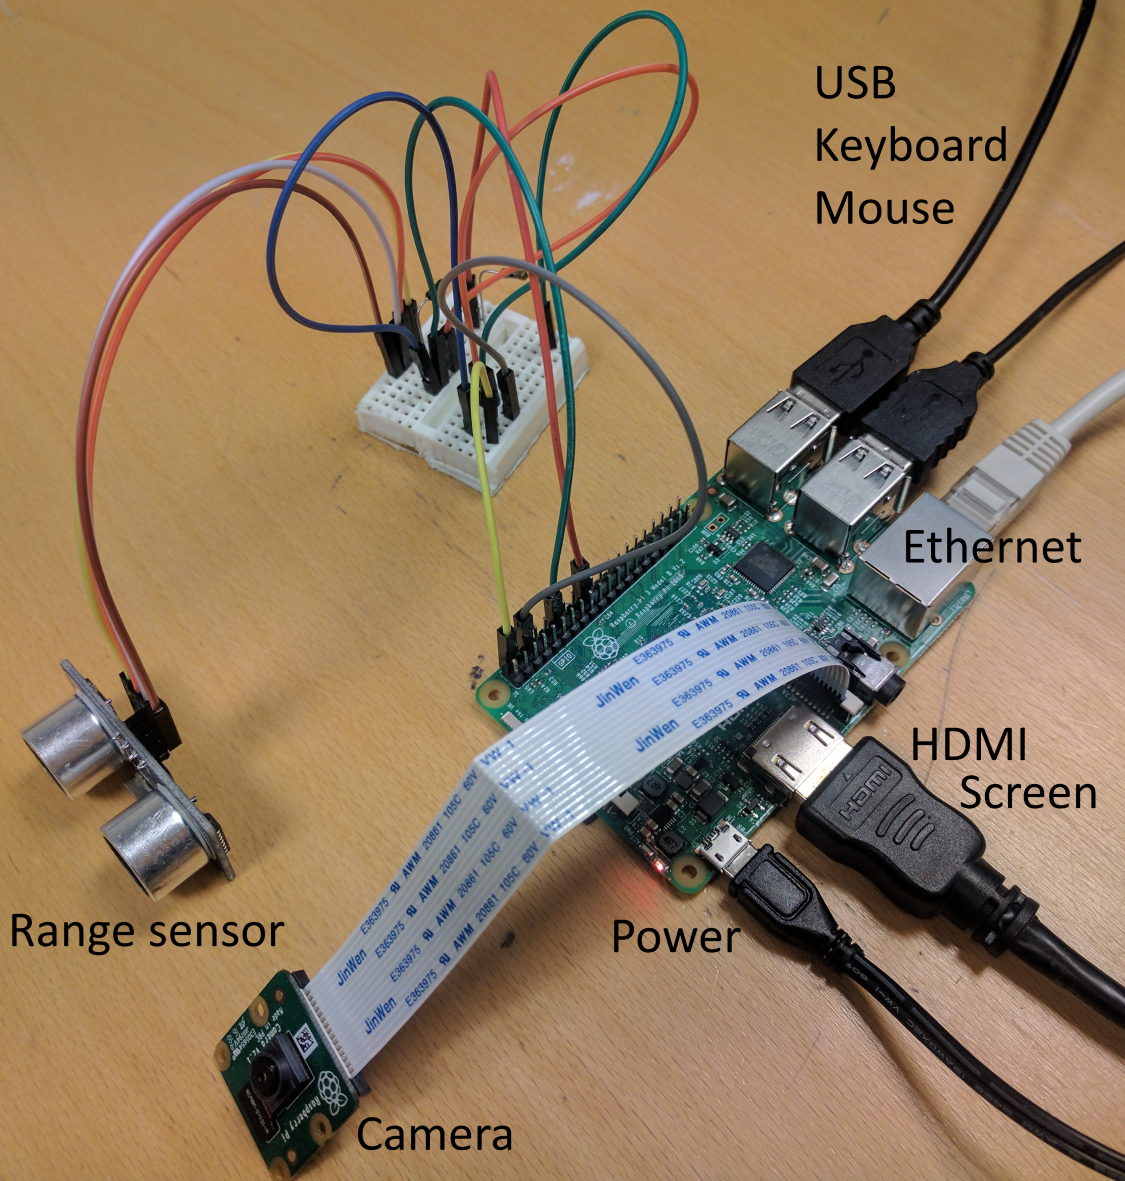
\includegraphics[width=0.85\textwidth]{fig/setup_debug}
  \caption{Debug hardware setup}
  \label{fig:setup_d}
\end{figure}

\subsection{Raspberry Pi}

\begin{figure}[H]
  \centering
  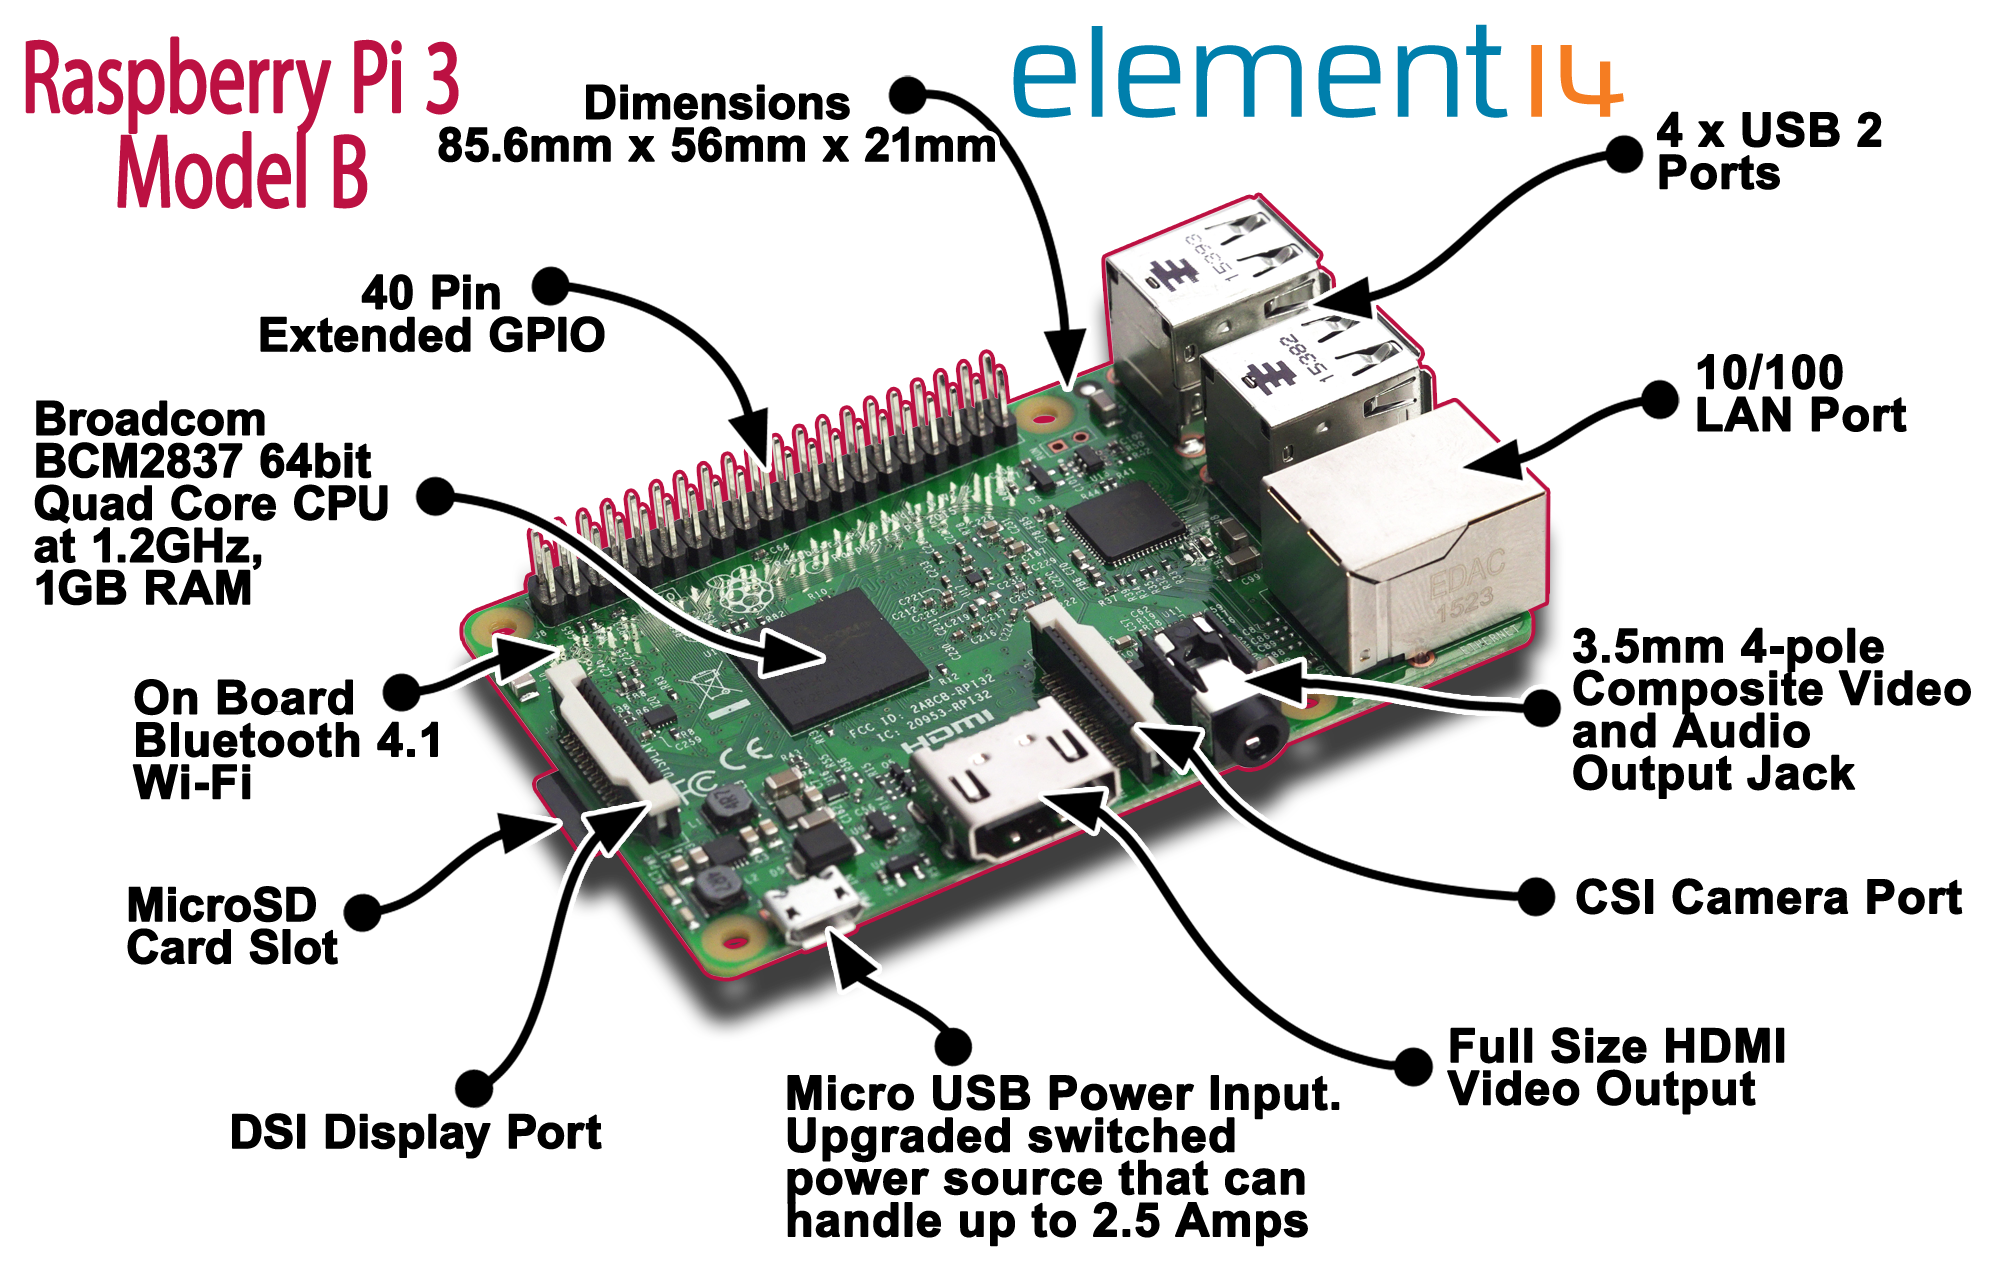
\includegraphics[width=1\textwidth]{fig/pi3}
  \caption{Raspberry Pi 3 Model B. \cite{pi3}}
  \label{fig:pi3}
\end{figure}

Figure \ref{fig:pi3} displays most of the I/O interfaces on the Raspberry Pi 3 Model B.

\begin{figure}[H]
  \centering
  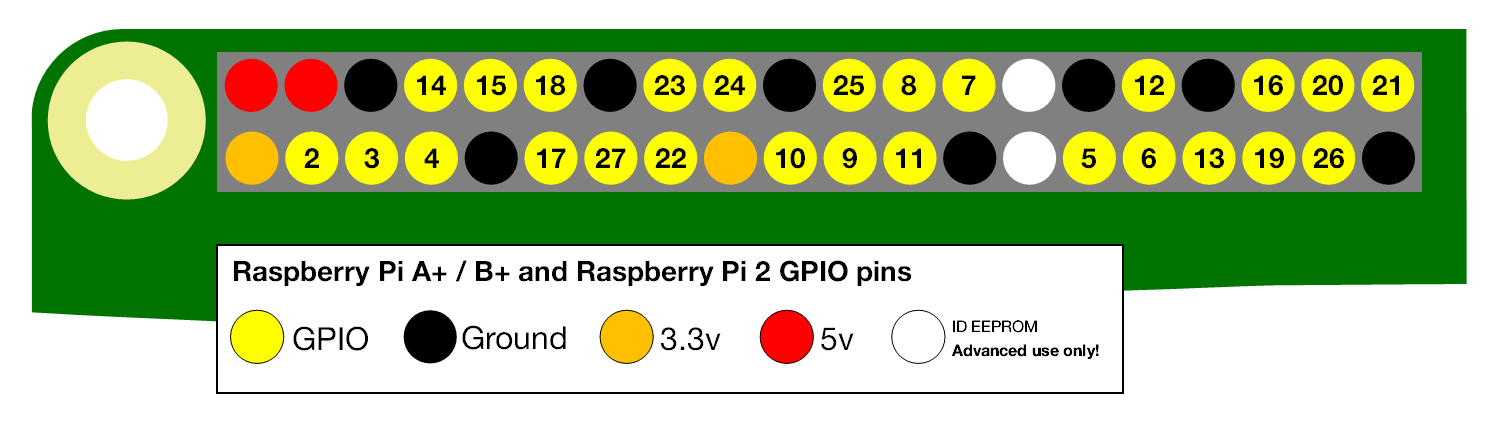
\includegraphics[width=1\textwidth]{fig/gpio}
  \caption{GPIO Pins on the Raspberry Pi 3\cite{rpi}}
  \label{fig:gpio}
\end{figure}

Figure \ref{fig:gpio} details the GPIO pins on the Raspberry Pi. This map is used to define the correct pins in the range sensor programming. 

\newpage
\subsection{Camera}
I am using the Raspberry Pi Camera v2 Module optimized for the Raspberry Pi. The camera includes a CSI cable that is connected to the Raspberry Pi through the CSI camera port on the board. The blue markings on the CSI cable should face the LAN port.

\begin{figure}[h]
  \centering
  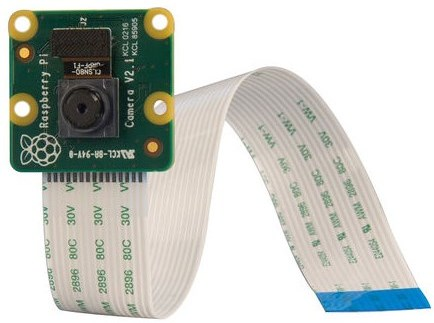
\includegraphics[width=0.6\textwidth]{fig/picam2}
  \caption{Raspberry Pi Camera Module V2 with CSI cable}
  \label{fig:picam2}
\end{figure}

\begin{figure}[h]
  \centering
  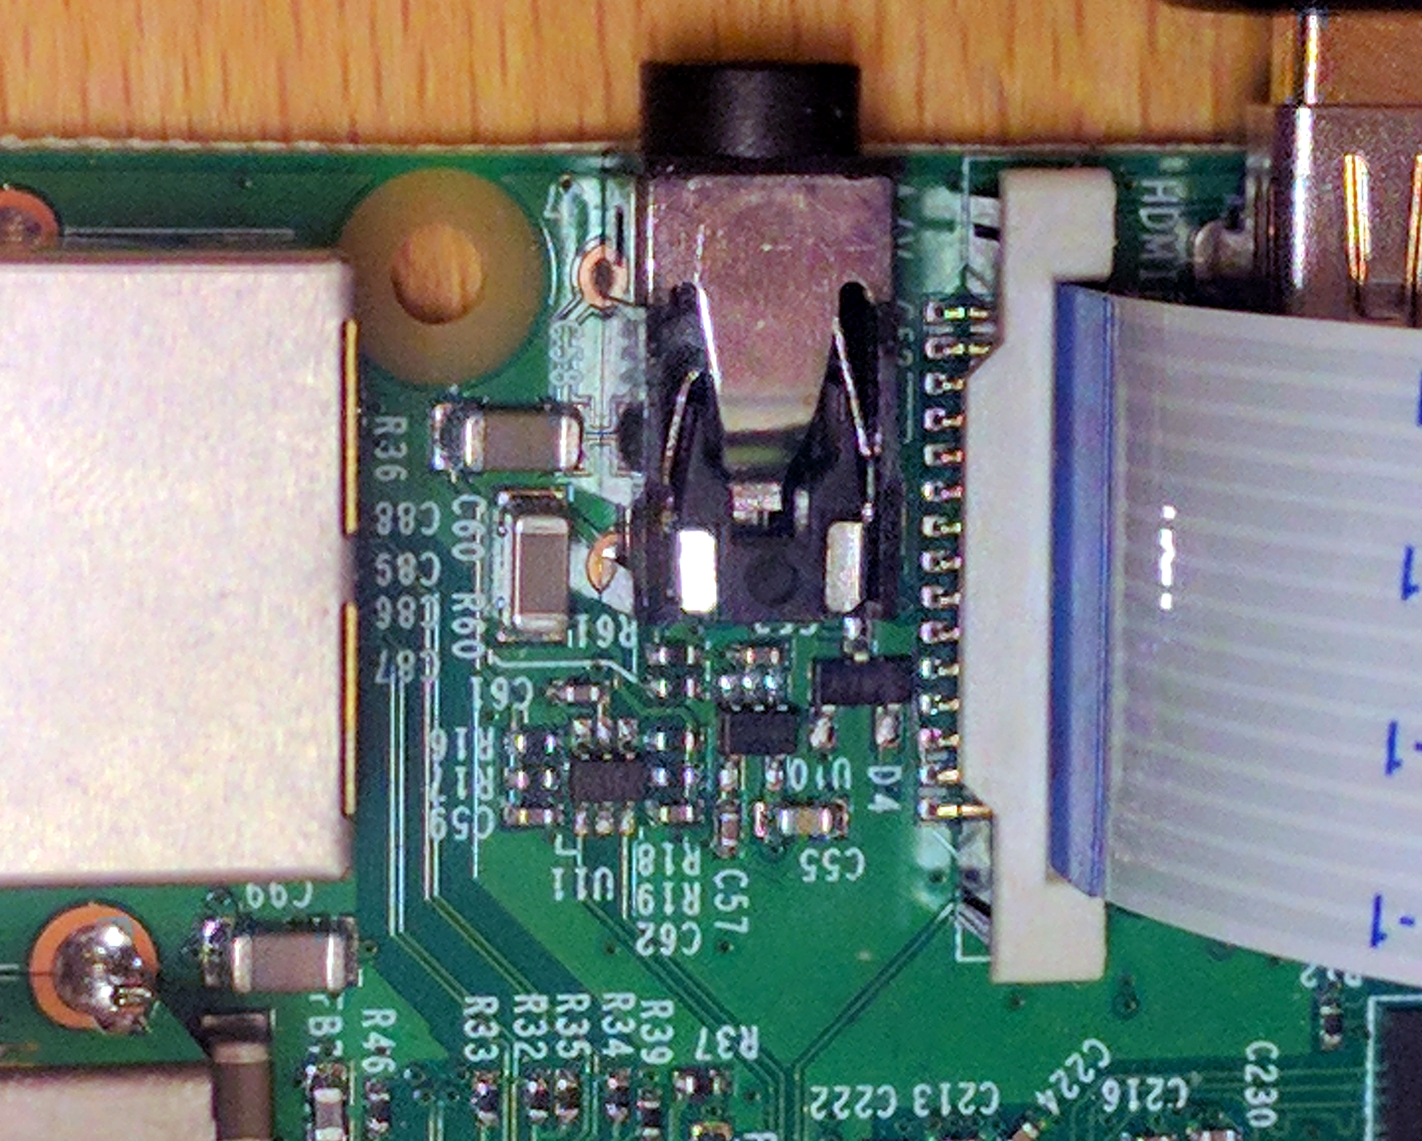
\includegraphics[width=0.6\textwidth]{fig/csi}
  \caption{CSI Cable mount}
  \label{fig:csi}
\end{figure}

\newpage
\subsection{Range sensor}
%LEGGE TID HVORDAN RANGE SENSOREN FUNKER MTP ECHO ETC
The HC-SR04 is a very easy sensor to use, but in order to make it compatible with the Raspberry Pi, there are some modifications needed. The GPIO input pins on the Raspberry Pi is made for 3.3V while the ECHO output pin on the HC-SR04 delivers 5V. So in order for the Raspberry Pi to interact with the HC-SR04, I need to reduce the voltage to 3.3V.\\

\begin{figure}[h]
  \centering
  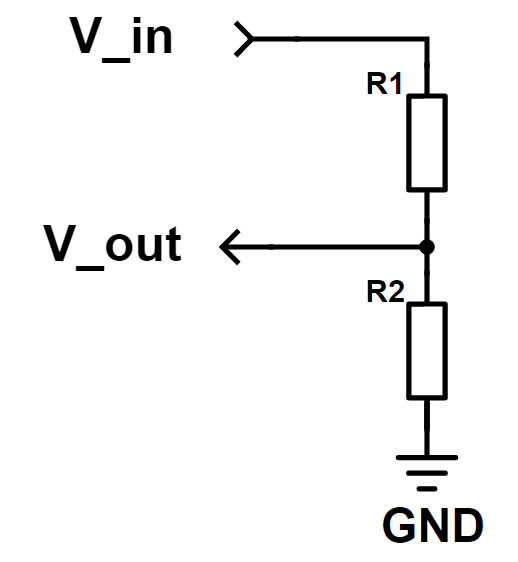
\includegraphics[width=0.3\textwidth]{fig/volt}
  \caption{Voltage divider}
  \label{fig:volt}
\end{figure}

This can be done with a simple voltage divider. Figure \ref{fig:volt} illustrates a simple voltage divider circuit that can be easily created with two resistors since we know the input and output voltages. The formula for a voltage divider is as follows:

\begin{align}
V_{out} = V_{in}\times \frac{R_2}{R_1 + R_2}
\end{align}

I want the $V_{out}$ to be 3.3V, and the $V_{in}$ is 5V. By a combination of resistors R1 and R2 the desired output voltage can be obtained. By picking R1$ = 820\Omega$ and R2$ = 1500\Omega$ we get:

\begin{align*}
V_{out} = 5 \times \frac{1500}{820+1500} = 3.23 V
\end{align*}

This is close enough for our application, and this is verified in the tests later in the thesis. Figure \ref{fig:rangesensor} shows how this voltage divider is implemented, and to which GPIO pins on the Raspberry Pi it is connected. Figure \ref{fig:hc2} shows the four pins on the HC-SR04.

\begin{figure}[H]
  \centering
  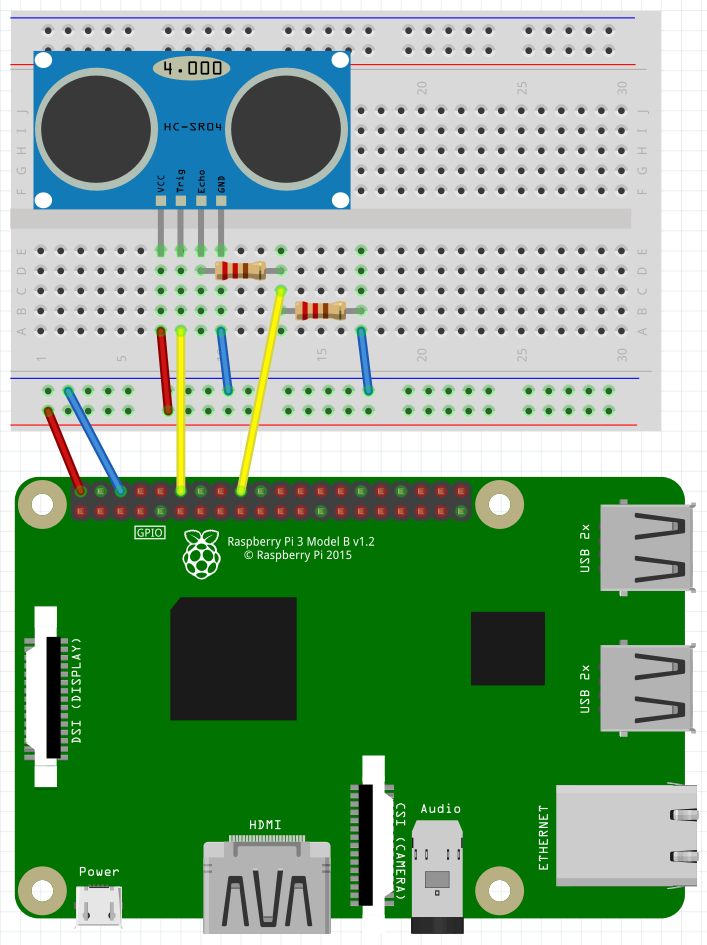
\includegraphics[width=0.6\textwidth]{fig/SensorSketch}
  \caption{Range sensor setup}
  \label{fig:rangesensor}
\end{figure}

\begin{figure}[H]
  \centering
  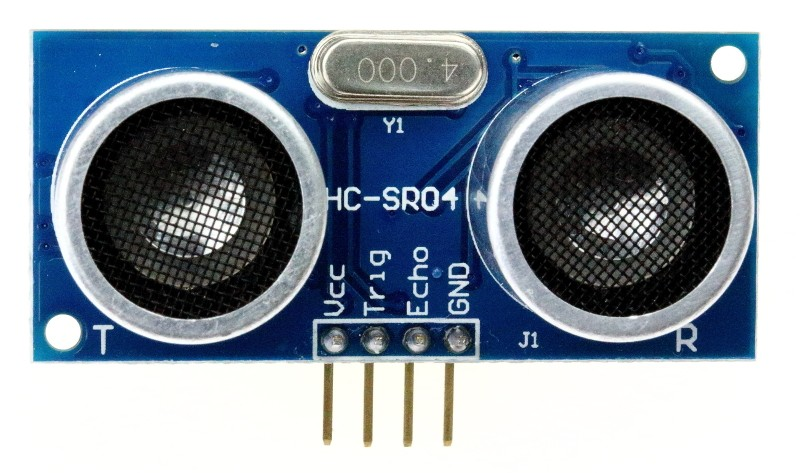
\includegraphics[width=0.6\textwidth]{fig/hc2}
  \caption{HC-SR04 pins. Vcc, Trig, Echo, GND}
  \label{fig:hc2}
\end{figure}

\subsection{3D printed case}
To make the system more compact and to facilitate for a better hardware implementation a 3D printed Raspberry Pi case was used. The case was collected from the Thingiverse library \cite{case}. \\

This case is designed so that the CSI cable and the GPIO pins can be accessed easily on the Raspberry Pi. The case was printed on a low-end off-the-shelf 3D printer.

\begin{figure}[H]
  \centering
  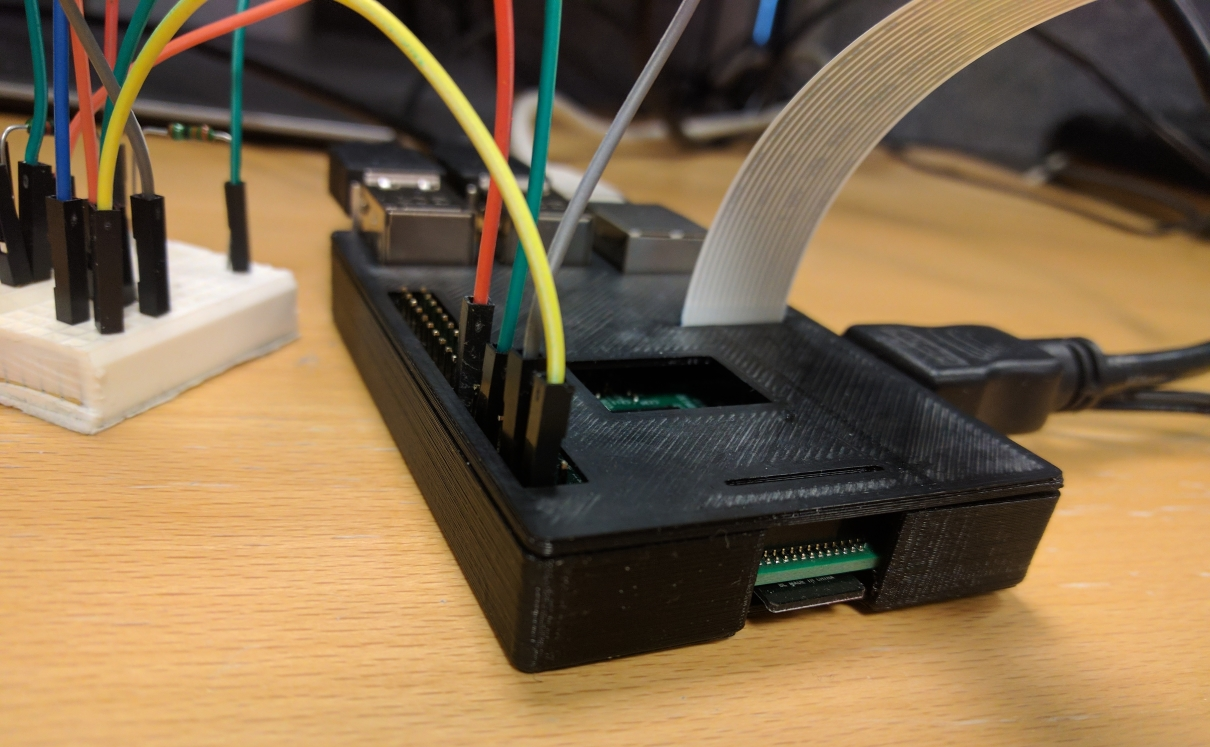
\includegraphics[width=1\textwidth]{fig/case}
  \caption{3D printed case}
  \label{fig:case}
\end{figure}












